\section*{Figures}
%\subsection*{Figure legends}

%\noindent Figure 1. Orca plots showing the temporal coverage of (A)
%catch/landings, (B) spawning stock biomass and (C) recruitment. The
%temporal coverage for individual assessments is represented by thin
%alternating black and grey horizontal lines in the main panels. Orca
%plots are named because their distinctive shape is uncannily similar
%to the individually-identifiable nicked and notched dorsal fins of
%killer whales (orcas). Thick horizontal lines at the base of each main
%panel represent the time periods which are present in 90\% (black) and
%50\% (grey) of all series for that data type.  Subfigure histograms
%contain the frequency of occurrence of the various timespans without
%reference to time period. Solid and long-dash vertical lines within
%the subfigures represent the median,
%2.5\% and 97.5\% quantiles, respectively.\\

%\noindent Figure 2. Map of Large Marine Ecosystems (LMEs) and
%high seas areas (ovals) showing the number of stock assessments
%present in the database for each area. This map illustrates the limited
%spatial coverage of available stock assessments.\\

%\noindent Figure 3. Comparison of the taxonomic diversity of marine
%species as provided by FishBase (top panel), the coverage of catch
%data as provided by the Sea Around Us database (middle panel) and the
%new RAM Legacy database (bottom panel). The circle located near the
%middle of the circular dendrogram represents kingdom Animalia and each
%subsequent branching represents a different taxonomic group (Kingdom
%to Phylum to Class to Order to Family to Genus to Species). The width
%of each line is proportional to the square root of the number of
%species in a branch. To facilitate the identification of the taxonomic
%groups that are not presented in the catch and assessment data, the
%FishBase branching pattern of the spoked dendrogram is maintained to
%generate the other two dendrograms.  This figure only compares fish
%and elasmobranch species present in FishBase. Additonal species of
%molluscs and arthropods are present in both the Sea Around Us and RAM
%Legacy databases but are not presented here.
%\\


%\noindent Figure 4. Current exploitation rate versus current biomass
%for 213 individual stocks and for individual stocks grouped by
%management unit. Exploitation is scaled relative to that which should
%allow maximum sustainable yield ($U_{msy}$); biomass is scaled
%relative to $B_{msy}$. Shades of grey indicate probability of
%occurrence as revealed by a kernel density smooth function. Solid
%circles indicate $B_{msy}$ and $U_{msy}$ that were obtained directly
%from assessments; open circles indicate that they were estimated from
%surplus production models. The panel labelled ``Atlantic'' includes
%ICCAT and NAFO. This figure is an updated version of Fig 3B from
%\citet{Worm:etal:2009:science}.
%\\

%\noindent Figure 5. Current exploitation rate versus current biomass grouped by the six taxonomic orders with the most assessments.
%\\

%\noindent Figure 6. Current exploitation rate versus current biomass grouped by mean trophic level.
%\\

%\newpage
\subsection*{Figures}

\begin{landscape}
\begin{figure}
\begin{center}
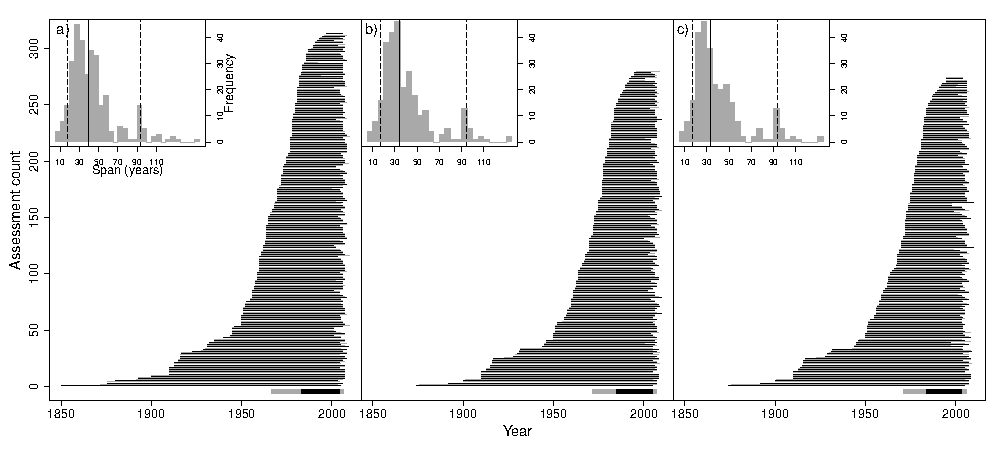
\includegraphics[width=8in]{/home/srdbadmin/srdb/projects/fishandfisheries/R/first-review/orca-plot.pdf}
\end{center}
\caption{ }\label{fig:orca}
\end{figure}
\end{landscape}

\begin{landscape}
\begin{figure}
\begin{center}
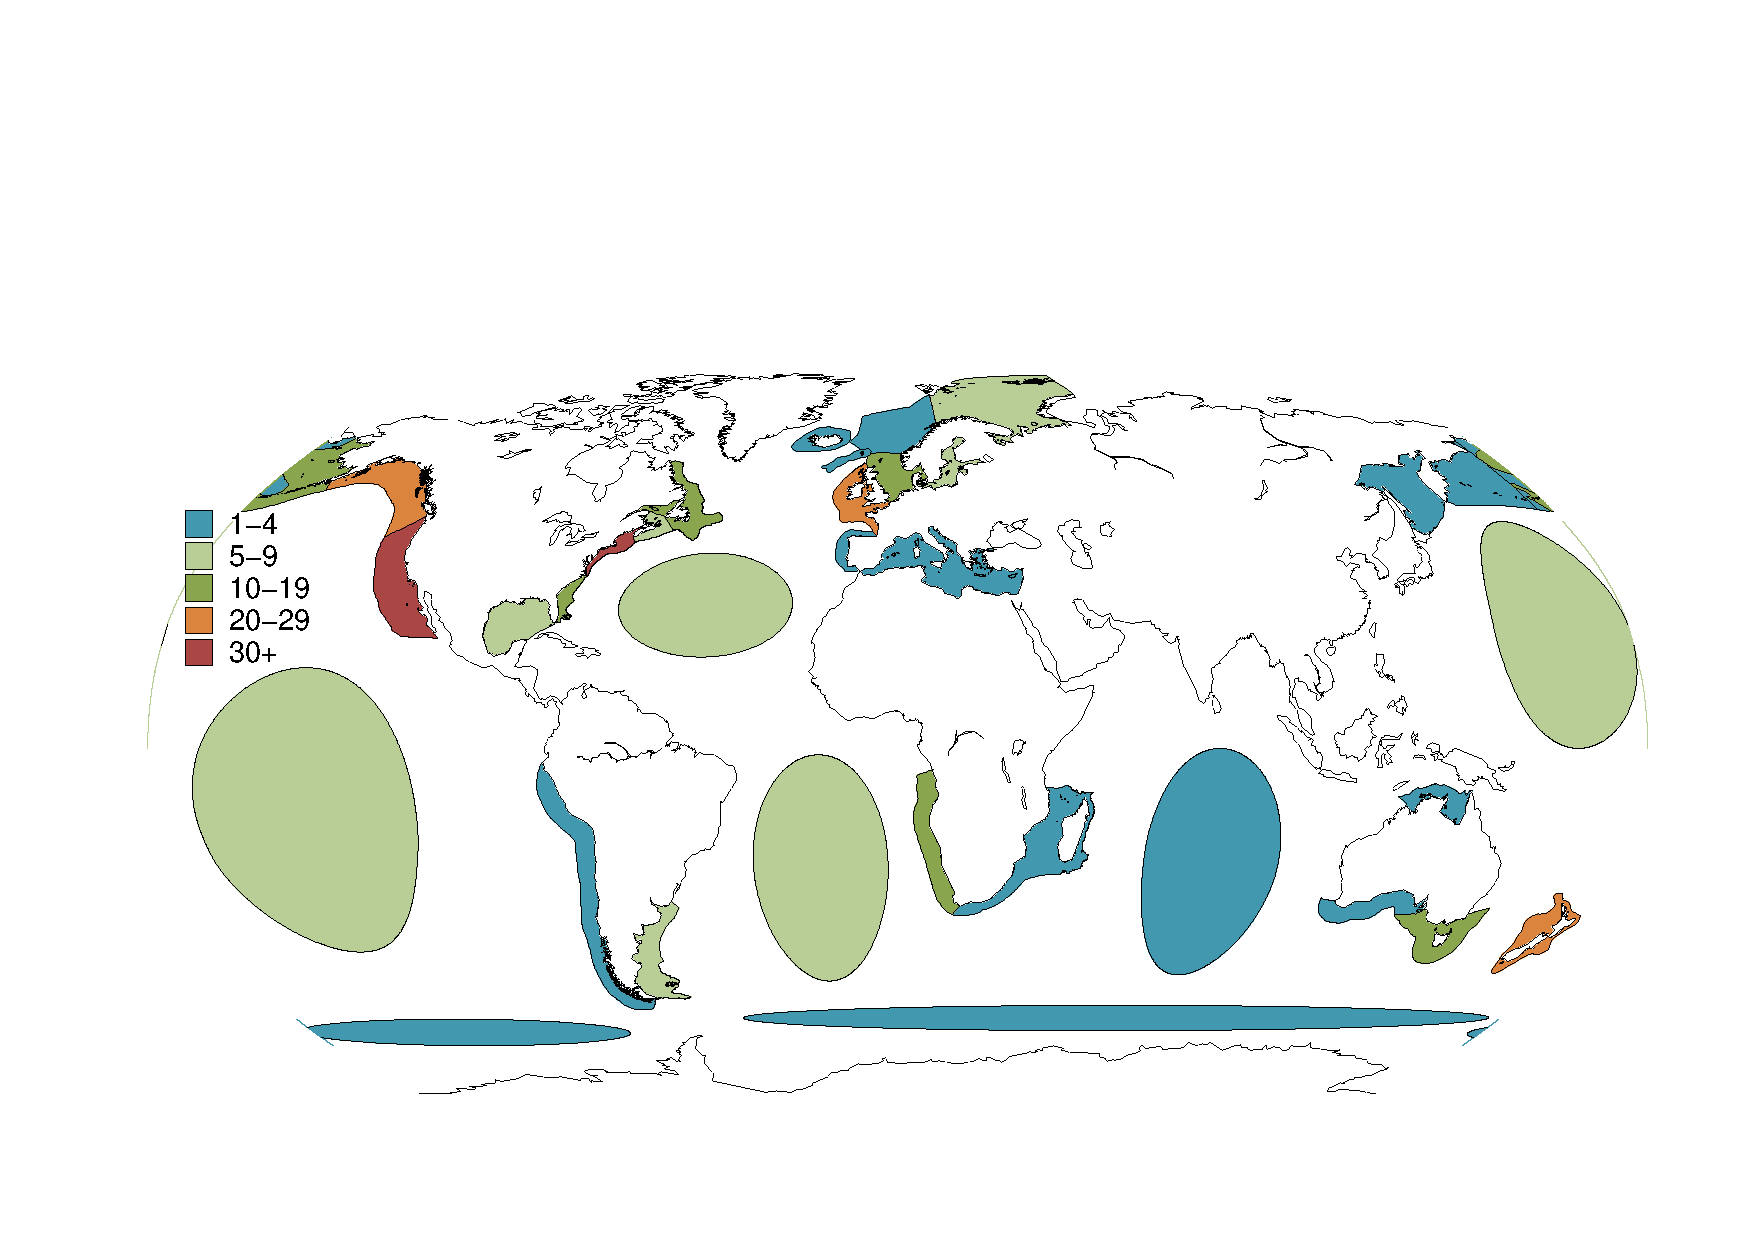
\includegraphics[width=9in]{/home/srdbadmin/srdb/projects/fishandfisheries/GMT/stocks-byLME.pdf}
\end{center}
\caption{ }\label{fig:lmes}
\end{figure}
\end{landscape}


\begin{figure}
\begin{center}
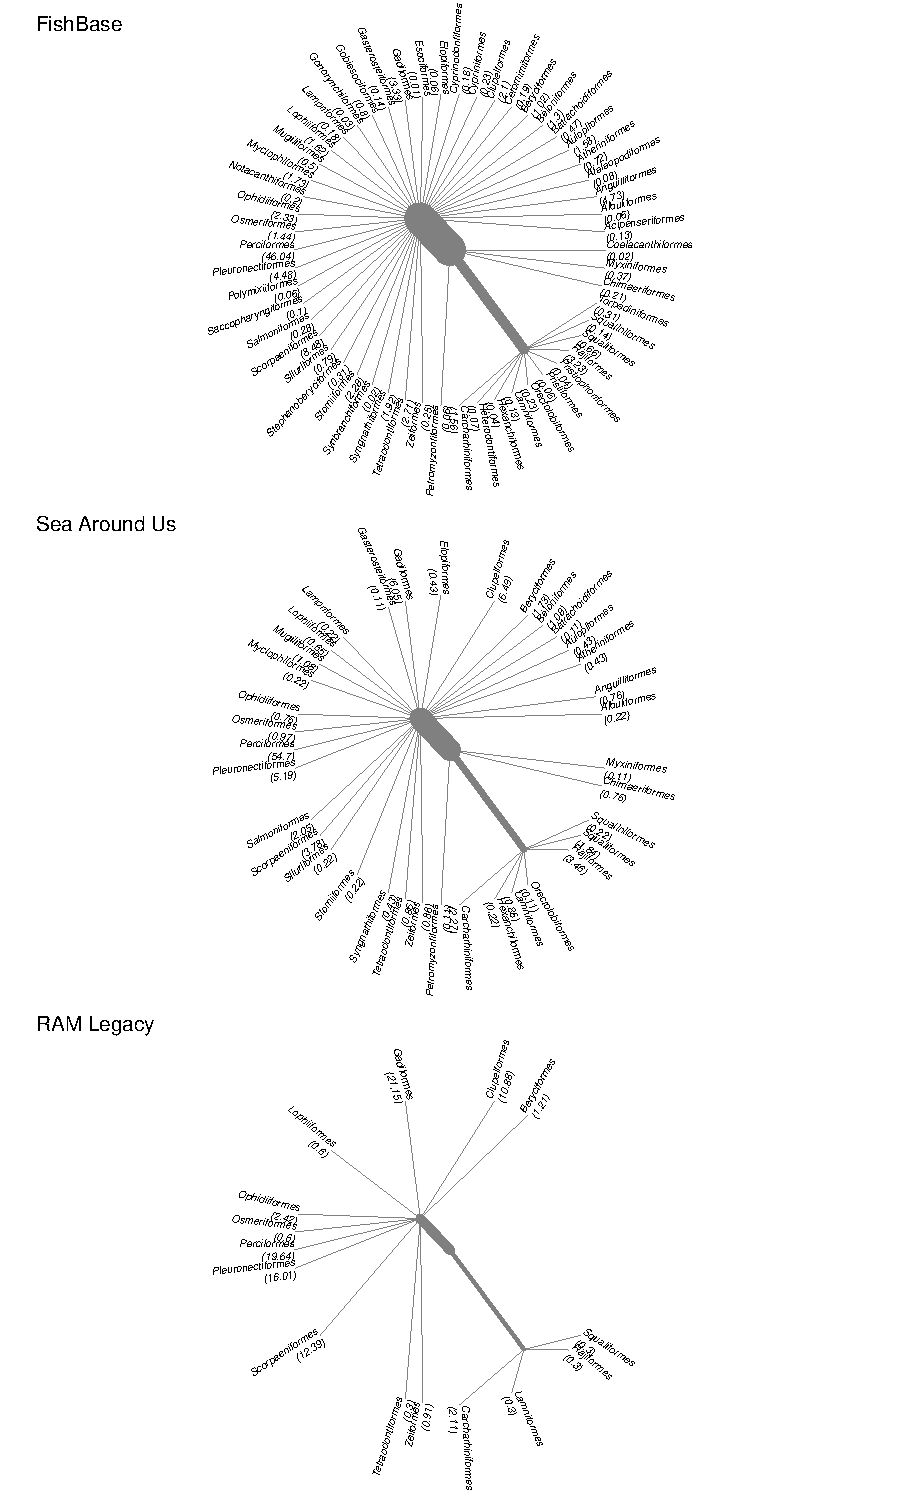
\includegraphics[height=8.5in]{/home/srdbadmin/srdb/projects/fishandfisheries/R/first-review/three-panel-phylo.pdf} % fishbase_saup_two_panel_phylo.pdf}
\end{center}
\caption{ }\label{fig:taxo:threepanel}
\end{figure}


\begin{landscape}
\begin{figure}
\begin{center}
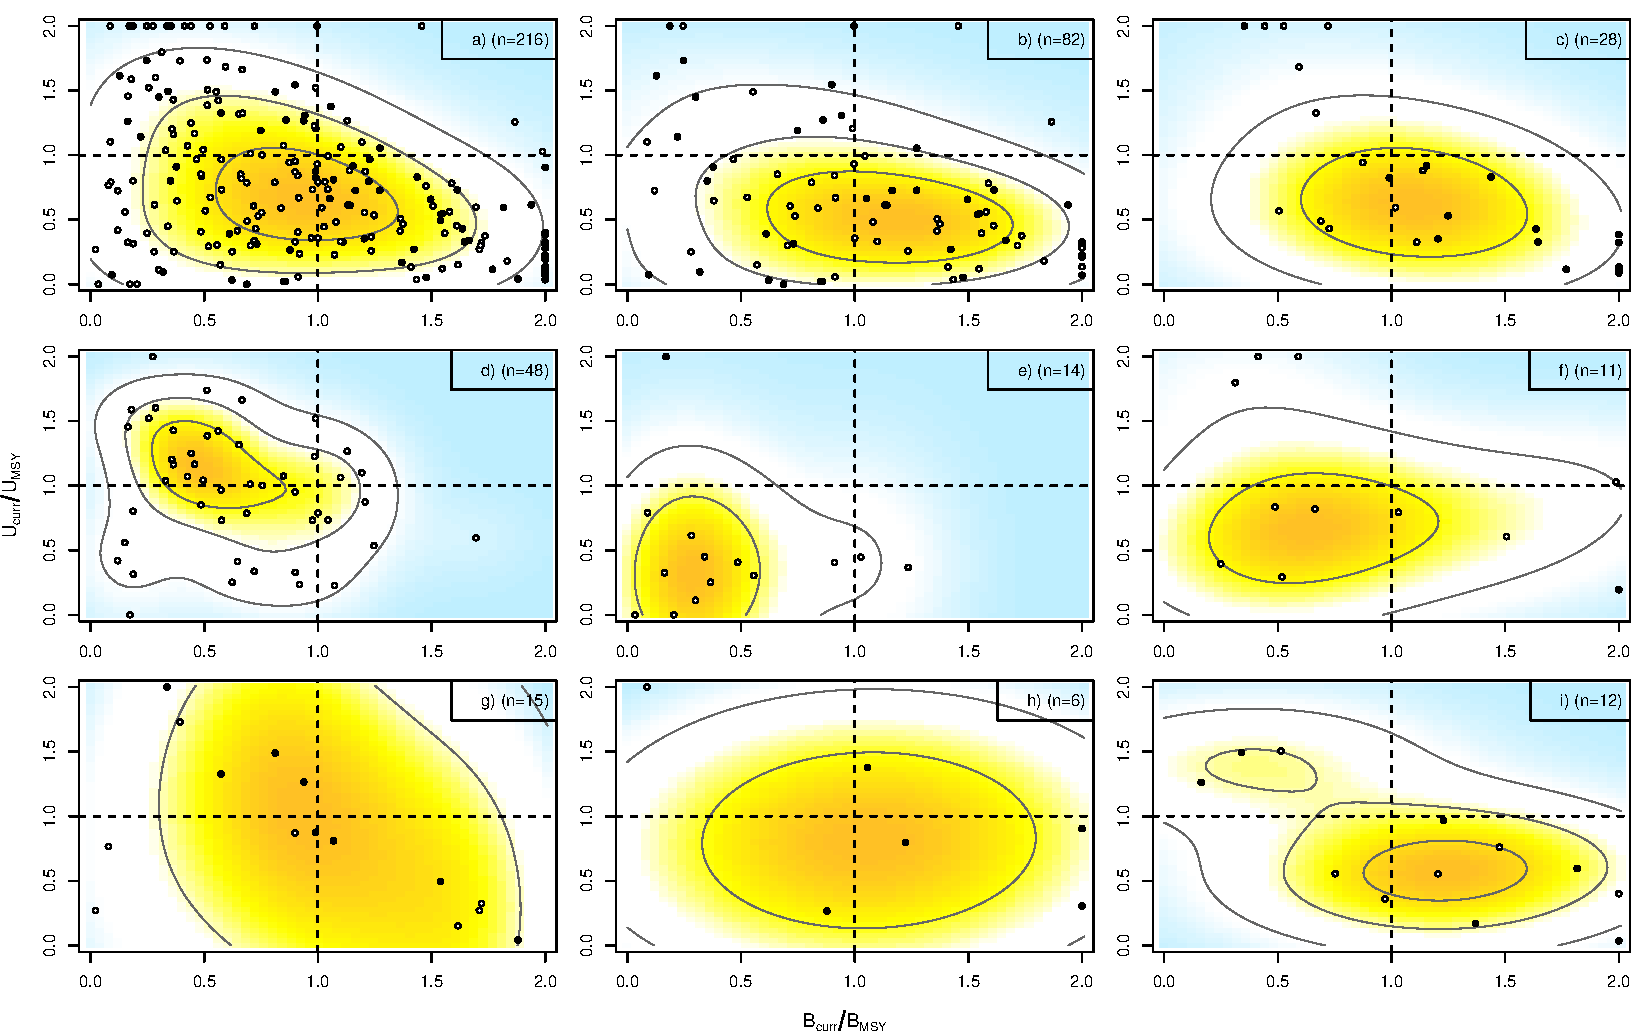
\includegraphics[width=9in]{/home/srdbadmin/srdb/projects/fishandfisheries/R/first-review/friedegg-9plots-fandf.pdf}
\end{center}
\caption{ }\label{fig:friedegg}
\end{figure}
\end{landscape}

%For the top 6 taxonomic orders (Figure~\ref{fig:taxo}).
\begin{figure}
\begin{center}
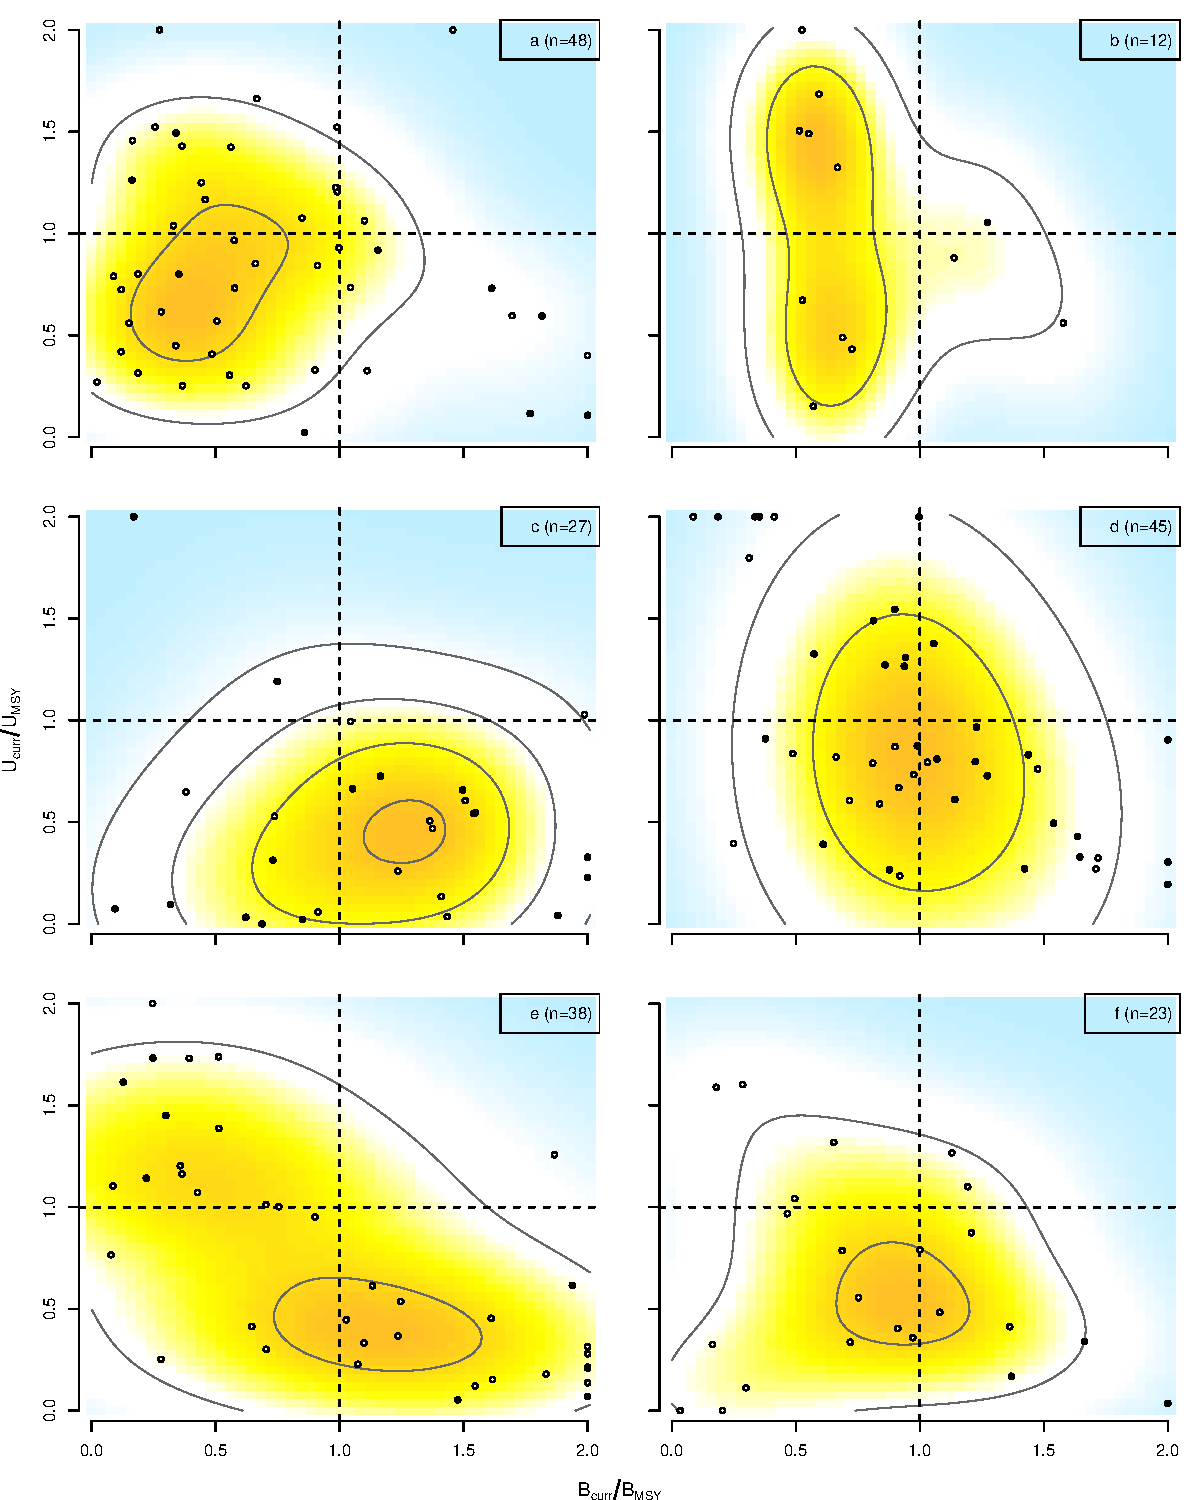
\includegraphics[width=15cm]{/home/srdbadmin/srdb/projects/fishandfisheries/R/first-review/friedegg-taxo.pdf}
\end{center}
\caption{ }
\label{fig:taxo}
\end{figure}

%By trophic level (Figure~\ref{fig:mtl}).
\begin{figure}
\begin{center}
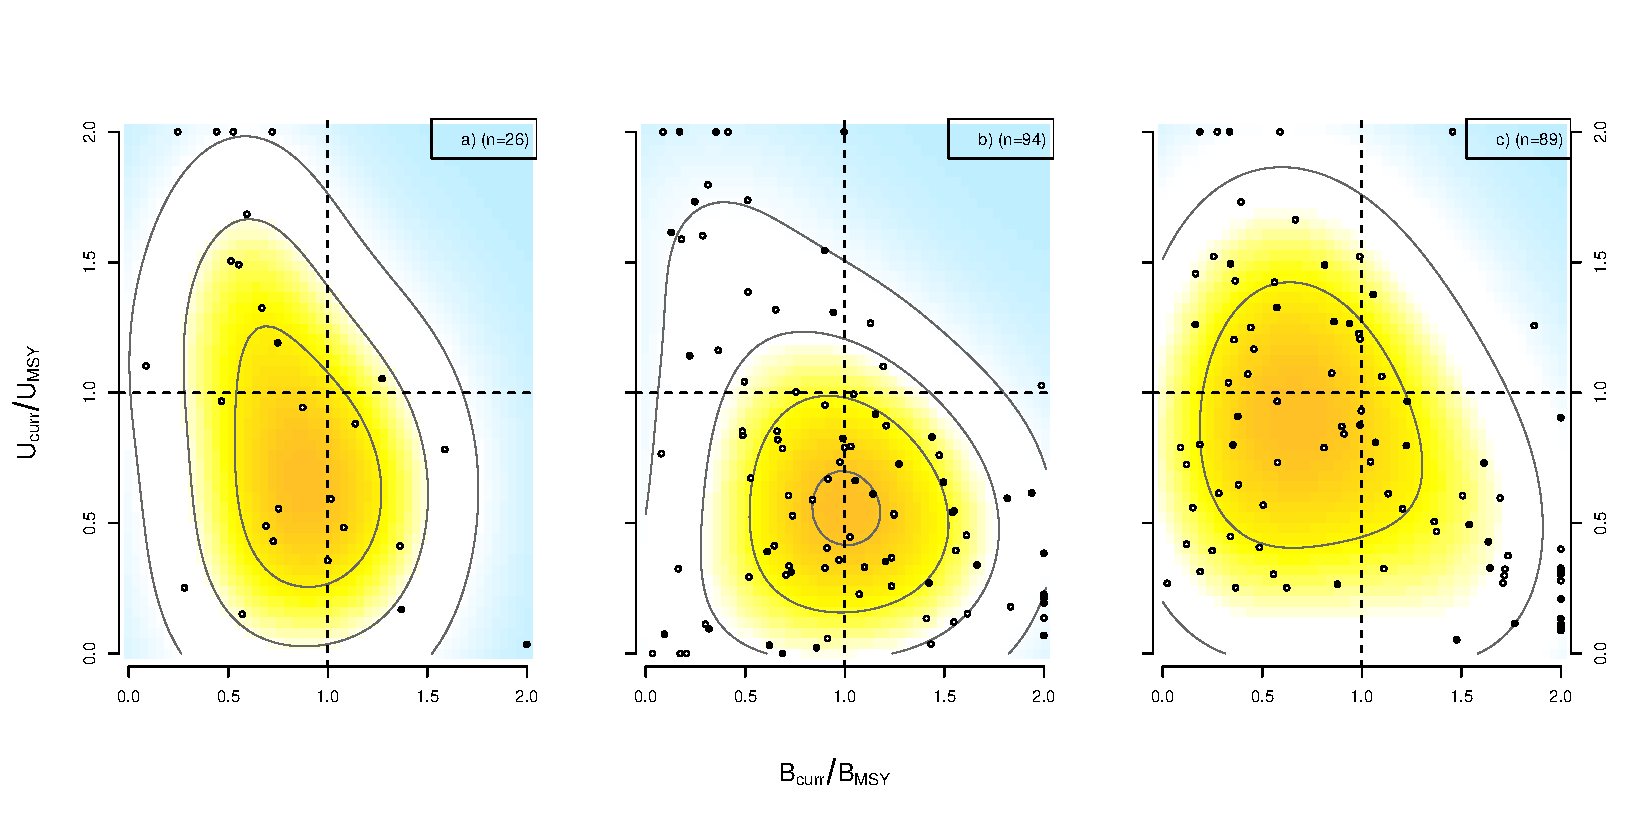
\includegraphics[width=15cm]{/home/srdbadmin/srdb/projects/fishandfisheries/R/first-review/friedegg-MTLs.pdf}
\end{center}
\caption{ }
\label{fig:mtl}
\end{figure}





